% ---------------------------------------------------------------------------------------------------
\section{Data Analysis}

% ---------------------------------------------------------------------------------------------------
\subsection{The dataset}
The dataset consists of $5110$ entries. Each entry correspond to one person's personal and medical 
information. A representation of the first entries of the dataset is presented in figure 
\ref{dataset_head}. The attributes, their possible values and frequencies are presented in tables 
\ref{table_attributes_1} and \ref{table_attributes_2}.


\begin{figure}[H]
\centering
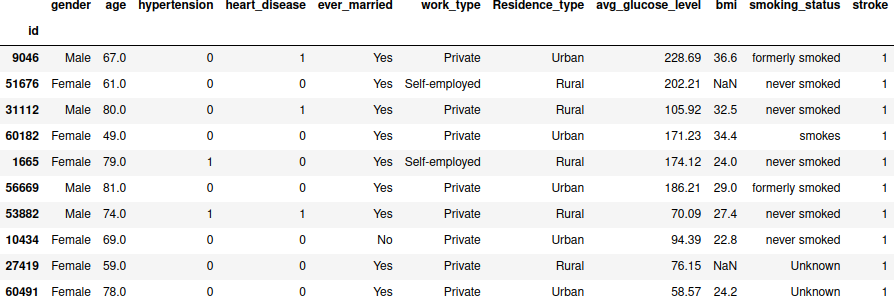
\includegraphics[scale=0.5]{figures/dataset_head.png}
\caption{dataset head}
\label{dataset_head}
\end{figure}

\begin{table}[H]\begin{tabular}{rm{11cm}}
 \textbf{id} & Unique patient identifier\\
 \textbf{gender} & Patient's gender\\
 \textbf{age} & Age of the patient\\
 \textbf{hypertension}   & Whether or not the patient has hypertension\\
 \textbf{heart\_disease} & Whether or not the patient has a heart disease\\
 \textbf{ever\_married} & Whether or not the patient is married\\
 \textbf{work\_type} & Work status of the patient\\
 \textbf{Residence\_type} & Residence type of the patient\\
 \textbf{avg\_glucose\_level} & Patient's average glucose level in the blood\\
 \textbf{bmi} & Patient's body mass index\\
 \textbf{smoking\_status} & Patient's smoking status\\
 \textbf{stroke} & Whether or not the patient had a stroke
\end{tabular}
\caption{Dataset attributes}
\label{table_attributes_1}
\end{table}

\begin{table}[H]\begin{tabular}{rcm{11cm}}
\textbf{Attribute} & \textbf{C/N} & \textbf{Value (frequency)}\\\hline\hline
gender             & C & Male (2115), Female (2994), Other (1)\\
age                & N & \# (5110)\\
hypertension       & C & 0 (4612), 1 (498)\\
heart\_desease     & C & 0 (4834), 1 (276)\\
ever\_married      & C & Yes (3353), No (1756)\\
work\_type         & C & Private (2925), Self-employed (819), Govt\_job (657), children (687), Never\_worked(22)\\
residence\_type    & C & Rural (2514), Urban (2596) \\
avg\_glucose\_level& N & \# (5110)\\
bmi                & N & \# (4909)\\
smoking\_status    & C & formerly smoked (884), never smoked (1892), smokes (789), Unknown (1544)\\
stroke             & C & 0 (5861), 1 (249)\\
\end{tabular}
\caption{Table of the attributes of the dataset with their categorical (C) or numerical (N) possible values.}
\label{table_attributes_2}
\end{table}

% ---------------------------------------------------------------------------------------------------
\subsection{Searching for outliers}
The distribution of the numerical attributes enables the search of possible data outliers that could 
alter the analysis. Figures \ref{dataset_describe} and \ref{hist_plots} present statistics and 
distribution of numerical attributes. The numerical attributes are of interest : 'age', 
'avg\_glucose\_level' and 'bmi'. \\

The standard deviation of these attributes is always small compared to the mean which implies no 
presence of outlier values. The plot distribution confirms this observation (figure \ref{hist_plots}) 
for 'age' and 'avg\_glucose\_level' attributes. However, few values of BMI greater than 60 seems out 
of scale and are outliers. A body mass index of 60 is considered as hyper-obesity and is relatively 
rare but possible condition. These date could be kept as true data. Cases of hyper-hyper-obesity 
(bmi > 80) are however extremely rare and could be errors in the measurements. Figure \ref{large_bmi} 
presents the entries of the dataset where bmi is greater than 90.

\begin{figure}[H]
\centering
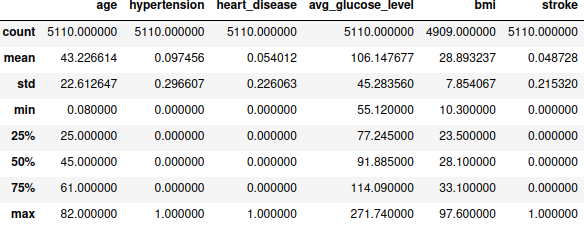
\includegraphics[scale=0.6]{figures/dataset_describe.png}
\caption{Statistics on numerical attributes of the dataset.}
\label{dataset_describe}
\end{figure}


\begin{figure}[H]
\centering
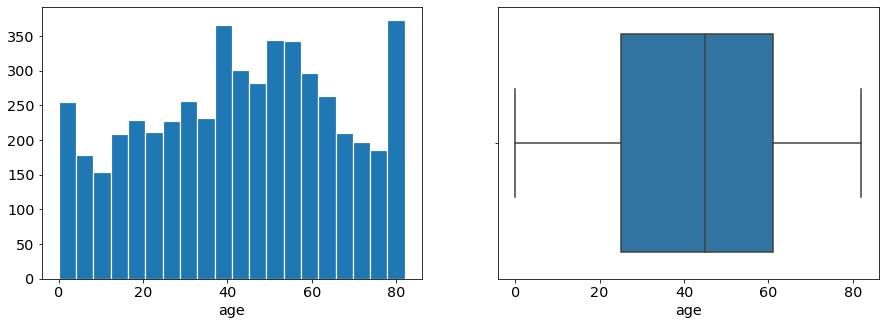
\includegraphics[scale=0.3]{../figures/hist_boxplot_age.png}\\
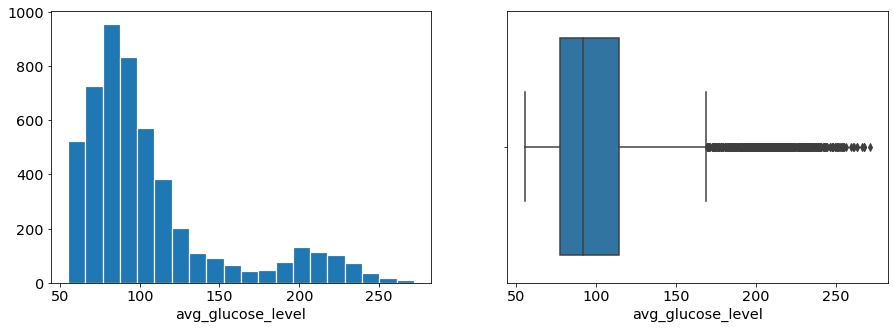
\includegraphics[scale=0.3]{../figures/hist_boxplot_avg_glucose_level.png}\\
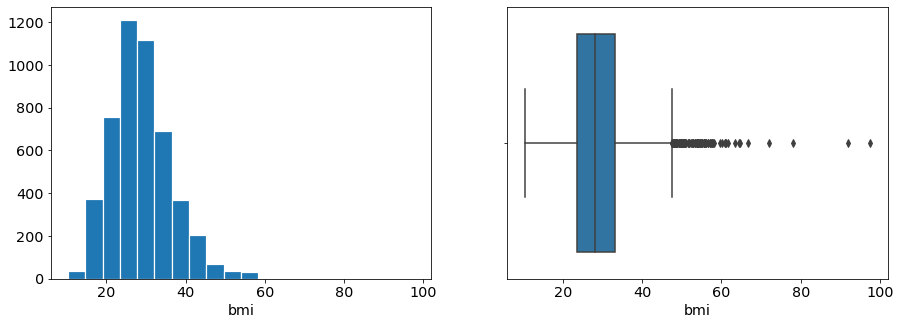
\includegraphics[scale=0.3]{../figures/hist_boxplot_bmi.png}
\caption{Distribution of the attributes 'age' (first line), 'avg\_glucose\_level' (second line) and BMI (third line). Histograms (left column) with bin widths of 50 and box plot (right column) showing the quartiles.}
\label{hist_plots}
\end{figure}

\begin{figure}[H]
\centering
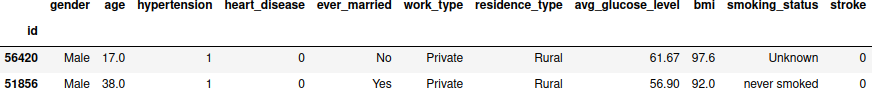
\includegraphics[scale=0.5]{figures/bmi_outliers_gt90.png}
\caption{Dataset entries where bmi is greater than 90.}
\label{large_bmi}
\end{figure}

% ---------------------------------------------------------------------------------------------------
\subsection{Missing values}
Figure \ref{dataset_describe} shows 201 missing values of bmi. The $1544$ 'Unknown' values of the 
'smoking\_status' attribute as well as one 'Other' value for the 'gender' attribute can also be 
considered as missing values. Section \ref{section_feature_engineering} on feature engineering will 
prsent how these missing values are handled.


% ---------------------------------------------------------------------------------------------------
\subsection{Class imbalance}
\label{section_imbalance}
Three attributes relating to heath issues ('stroke', 'heart\_disease' and 'hypertension') are 
bookean attributes. The figure \ref{pie_plots} presents the distribution of these attributes and 
show a dataset imbalance problem. Indeed, the 0 values are well more represented than the 1 values. 

\begin{figure}[H]
 \efbox{
  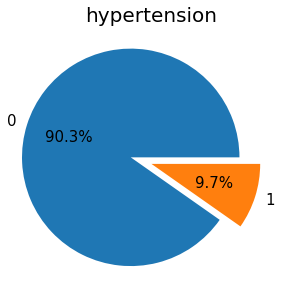
\includegraphics[scale=0.45]{../figures/pie_hypertension.png}
  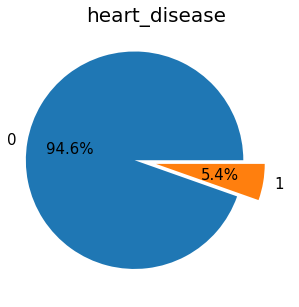
\includegraphics[scale=0.45]{../figures/pie_heart_disease.png}
  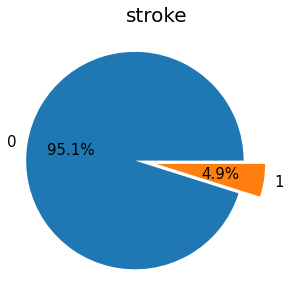
\includegraphics[scale=0.45]{../figures/pie_stroke.png}
  }
 \caption{Distribution of the values of the attributes 'hypertension', 'heart\_disease' and 'stroke'.}
 \label{pie_plots}
\end{figure}

Because this study is about the predectability of one patient having a stroke, the health attributes 
could have high impact in the modeling. The correlation between these attributes (figure 
\ref{figure_correlation_strokeHeartDiseaseHypertension}) seem however to suggest that they are only 
little correlated.

\begin{figure}[H]
\centering
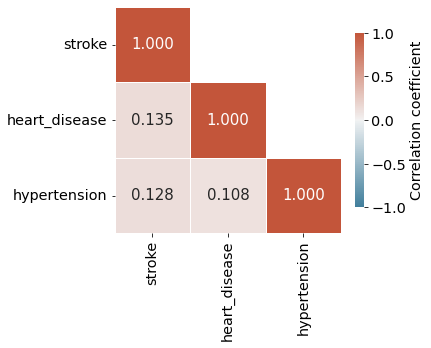
\includegraphics[scale=0.5]{../figures/correlationMatrix_strokeHeartDiseaseHypertension.png}
\caption{Correlation coefficients between the parameters 'stroke', 'heart\_disease' and 'hypertension'.}
\label{figure_correlation_strokeHeartDiseaseHypertension}
\end{figure}


% ---------------------------------------------------------------------------------------------------
\subsection{Attributes name consistency}
The attribute 'Residence\_type', starting with a capital letter, is renamed to 'residence\_type' so 
to have etymological consistency. Indeed, all attributes except 'Residence\_type' have names starting 
with a lower-case letter.
